\documentclass{standalone}
\usepackage{tikz}
\usetikzlibrary{decorations.pathreplacing} % For braces

\begin{document}

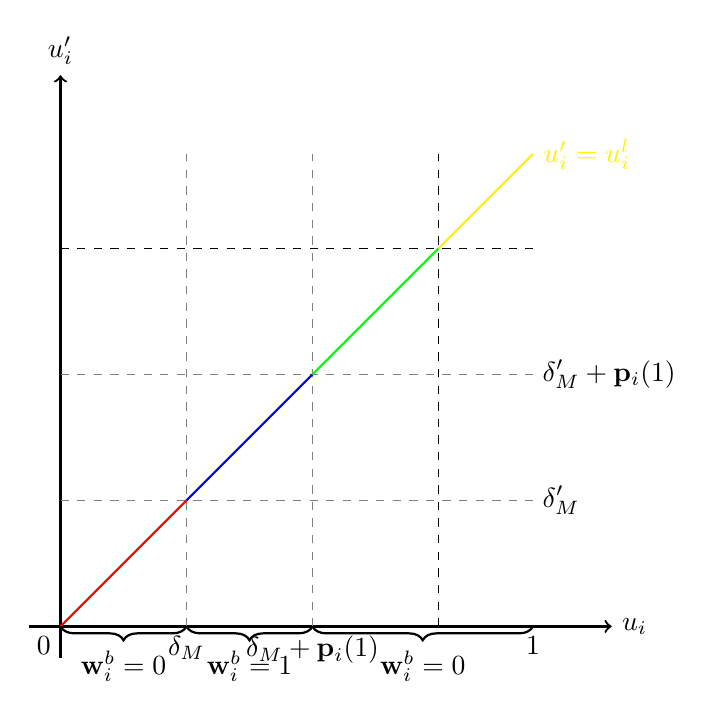
\begin{tikzpicture}[scale=2]

% Axes
\draw[->, thick] (-0.2, 0) -- (3.5, 0) node[right] {$u_i$};
\draw[->, thick] (0, -0.2) -- (0, 3.5) node[above] {$u_i'$};

% Dashed grid lines
\foreach \x in {0.8, 1.6, 2.4} {
    \draw[dashed] (\x, 0) -- (\x, 3);
}
\foreach \y in {0.8, 1.6, 2.4} {
    \draw[dashed] (0, \y) -- (3, \y);
}

% Horizontal dashed line at delta_M'
\draw[dashed, gray] (0, 1.6) -- (3, 1.6) node[right, black] {$\delta_M' + \mathbf{p}_i(1)$};
% Horizontal dashed line at delta_M
\draw[dashed, gray] (0, 0.8) -- (3, 0.8) node[right, black] {$\delta_M'$};

% Vertical dashed line at delta_M
\draw[dashed, gray] (0.8, 0) -- (0.8, 3) node[above, black] {};
% Vertical dashed line at delta_M + p_i(1)
\draw[dashed, gray] (1.6, 0) -- (1.6, 3) node[above, black] {};

% Red line segment
\draw[red, thick] (0, 0) -- (0.8, 0.8);

% Blue line segment
\draw[blue, thick] (0.8, 0.8) -- (1.6, 1.6);

% Green line segment
\draw[green, thick] (1.6, 1.6) -- (2.4, 2.4);

% Yellow line segment
\draw[yellow, thick] (2.4, 2.4) -- (3, 3) node[right] {$u_i' = u_i^l$};

% Braces for w^b_i labels
\draw[decorate, decoration={brace, mirror, amplitude=5pt}, thick] (0, 0) -- node[below=5pt] {$\mathbf{w}_i^b = 0$} (0.8, 0);
\draw[decorate, decoration={brace, mirror, amplitude=5pt}, thick] (0.8, 0) -- node[below=5pt] {$\mathbf{w}_i^b = 1$} (1.6, 0);
\draw[decorate, decoration={brace, mirror, amplitude=5pt}, thick] (1.6, 0) -- node[below=5pt] {$\mathbf{w}_i^b = 0$} (3, 0);

% Labels
\node[below left] at (0, 0) {$0$};
\node[below] at (0.8, 0) {$\delta_M$};
\node[below] at (1.6, 0) {$\delta_M + \mathbf{p}_i(1)$};
\node[below] at (3, 0) {$1$};
\node[left] at (0, 1.6) {};
\node[left] at (0, 0.8) {};

\end{tikzpicture}

\end{document}